% -*- coding: UTF-8 -*-
\documentclass{article}
\usepackage{amsmath}
\usepackage{tikz}


\begin{document}
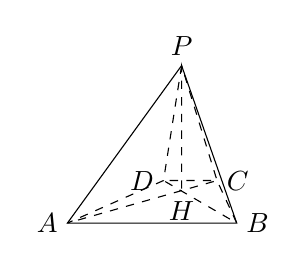
\begin{tikzpicture}

  \coordinate[label=180:$A$] (a) at (0,0);
  \coordinate[label=0:$B$] (b) at (2.15,0);
  \coordinate[label=0:$C$] (c) at (1.9,0.54);
  \coordinate[label=180:$D$] (d) at (1.22,0.54);
  \coordinate[label=-90:$H$] (h) at (1.45,0.4);
  \coordinate[label=90:$P$] (p) at (1.45,2);


  \draw (b) -- (a) -- (p) -- cycle;
  \draw[dashed] (p) -- (d) -- (a) -- (c) -- (b) -- (d) -- (c) -- (p) -- (h);

\end{tikzpicture}
\end{document}
